% !TEX program = xelatex
% ================================================================
% SLIDE TÓM TẮT VĂN BẢN TIẾNG VIỆT - BEAMER / OVERLEAF
% Biên dịch bằng XeLaTeX.
% Các vị trí cần cập nhật nhanh được gom trong khối "THÔNG TIN DỰ ÁN".
% ================================================================

\documentclass[aspectratio=169,10pt]{beamer}

% ---------- Ngôn ngữ, font và gói cơ bản ----------
\usepackage{fontspec}
\setsansfont{Latin Modern Sans}
\setmonofont{Latin Modern Mono}
\usefonttheme{professionalfonts}
\usepackage{amsmath,amssymb}
\usepackage{booktabs,tabularx,array,multirow}
\usepackage[table]{xcolor}
\usepackage{graphicx}
\usepackage{tikz}
\usepackage{pgfplots}
\pgfplotsset{compat=1.18}
\usepackage[most]{tcolorbox}
\usepackage{ragged2e}
\usepackage{microtype}
\usepackage{hyperref}

% ---------- THÔNG TIN DỰ ÁN: sửa tại đây ----------
\newcommand{\ProjectTitle}{Tóm tắt văn bản tiếng Việt}
\newcommand{\ProjectSubtitle}{So sánh Transformer Seq2Seq xây dựng từ đầu và ViT5}
\newcommand{\EnglishSubtitle}{Abstractive Text Summarization for Vietnamese News}
\newcommand{\MemberNames}{Trần Đức Thịnh \quad và \quad Lưu Xuân Tân}
% Ví dụ nếu nhóm có 4 người:
% \renewcommand{\MemberNames}{Trần Đức Thịnh \quad Lưu Xuân Tân \\ Thành viên 3 \quad Thành viên 4}
\newcommand{\UniversityName}{Đại học Công nghệ, ĐHQGHN}
\newcommand{\CourseName}{[Tên học phần]}
\newcommand{\TeacherName}{[Giảng viên hướng dẫn]}
\newcommand{\PresentationDate}{[Ngày thuyết trình]}

% ---------- KẾT QUẢ TEST: chỉ cần thay dấu -- bằng số ----------
\newcommand{\Pending}{\textcolor{gray!75}{--}}
\newcommand{\LeadOneRone}{\Pending}
\newcommand{\LeadOneRtwo}{\Pending}
\newcommand{\LeadOneRl}{\Pending}
\newcommand{\LeadOneCr}{\Pending}
\newcommand{\LeadThreeRone}{\Pending}
\newcommand{\LeadThreeRtwo}{\Pending}
\newcommand{\LeadThreeRl}{\Pending}
\newcommand{\LeadThreeCr}{\Pending}
\newcommand{\ScratchRone}{\Pending}
\newcommand{\ScratchRtwo}{\Pending}
\newcommand{\ScratchRl}{\Pending}
\newcommand{\ScratchCr}{\Pending}
\newcommand{\VitFiveRone}{\Pending}
\newcommand{\VitFiveRtwo}{\Pending}
\newcommand{\VitFiveRl}{\Pending}
\newcommand{\VitFiveCr}{\Pending}

% ---------- Hệ màu bám sát slide mẫu ----------
\definecolor{DeepBlue}{HTML}{003B6F}
\definecolor{NavyBlue}{HTML}{002F5D}
\definecolor{AccentRed}{HTML}{C31F26}
\definecolor{SoftRed}{HTML}{FFF0F0}
\definecolor{SoftBlue}{HTML}{E8F1FB}
\definecolor{SoftGreen}{HTML}{EAF8E7}
\definecolor{GoodGreen}{HTML}{138A36}
\definecolor{SoftYellow}{HTML}{FFF4B8}
\definecolor{MutedGray}{HTML}{5D6670}
\definecolor{LightGray}{HTML}{F3F5F7}
\definecolor{MidBlue}{HTML}{4D79A7}
\definecolor{VitPurple}{HTML}{6D66C2}

\hypersetup{colorlinks=true,urlcolor=DeepBlue,linkcolor=DeepBlue}

% ---------- Thiết lập Beamer ----------
\setbeamertemplate{navigation symbols}{}
\setbeamercolor{normal text}{fg=black!78,bg=white}
\setbeamercolor{frametitle}{fg=white,bg=DeepBlue}
\setbeamerfont{frametitle}{size=\Large,series=\bfseries}
\setbeamerfont{title}{size=\LARGE,series=\bfseries}
\setbeamerfont{subtitle}{size=\large}
\setbeamerfont{footline}{size=\tiny}
\setbeamercolor{structure}{fg=DeepBlue}
\setbeamercolor{itemize item}{fg=DeepBlue}
\setbeamercolor{itemize subitem}{fg=MidBlue}
\setbeamersize{text margin left=0.58cm,text margin right=0.58cm}

\setbeamertemplate{itemize item}{\raise0.15ex\hbox{\color{DeepBlue}\scriptsize$\blacktriangleright$}}
\setbeamertemplate{itemize subitem}{\raise0.1ex\hbox{\color{MidBlue}\tiny$\blacktriangleright$}}
\setlength{\leftmargini}{1.25em}
\setlength{\leftmarginii}{1.10em}

\setbeamertemplate{frametitle}{%
  \nointerlineskip
  \begin{beamercolorbox}[wd=\paperwidth,ht=0.78cm,dp=0.18cm,leftskip=0.38cm]{frametitle}
    \usebeamerfont{frametitle}\insertframetitle
  \end{beamercolorbox}%
}

\setbeamertemplate{footline}{%
  \leavevmode
  \hbox{%
    \begin{beamercolorbox}[wd=.90\paperwidth,ht=0.25cm,dp=0.08cm,leftskip=0.16cm]{frametitle}
      \usebeamerfont{footline}Transformer Seq2Seq và ViT5 cho Tóm tắt tiếng Việt \;|\; \MemberNames
    \end{beamercolorbox}%
    \begin{beamercolorbox}[wd=.10\paperwidth,ht=0.25cm,dp=0.08cm,rightskip=0.14cm plus 1fil]{frametitle}
      \usebeamerfont{footline}\hfill\insertframenumber/\inserttotalframenumber
    \end{beamercolorbox}%
  }%
}

\setbeamertemplate{headline}{}

% ---------- Thành phần dùng lại ----------
\newtcolorbox{keymessage}[1][Thông điệp chính]{
  enhanced,
  colback=SoftRed,
  colframe=AccentRed,
  colbacktitle=AccentRed,
  coltitle=white,
  fonttitle=\bfseries\scriptsize,
  fontupper=\small,
  title=#1,
  boxrule=0.7pt,
  arc=1mm,
  left=1.6mm,right=1.6mm,top=1.0mm,bottom=1.0mm,
  toptitle=0.5mm,bottomtitle=0.5mm
}

\newtcolorbox{softbox}[1][]{
  enhanced,
  colback=SoftBlue,
  colframe=DeepBlue,
  boxrule=0.6pt,
  arc=1mm,
  left=1.7mm,right=1.7mm,top=1.2mm,bottom=1.2mm,
  #1
}

\newtcolorbox{greenbox}[1][]{
  enhanced,
  colback=SoftGreen,
  colframe=GoodGreen,
  boxrule=0.7pt,
  arc=1mm,
  left=1.7mm,right=1.7mm,top=1.2mm,bottom=1.2mm,
  #1
}

% Tự chèn hình nếu file tồn tại; nếu chưa có thì hiện khung trống.
% #1 = chiều rộng, #2 = đường dẫn file, #3 = chiều cao, #4 = nhãn gợi ý.
\newcommand{\maybeimage}[4][\linewidth]{%
  \IfFileExists{#2}{%
    \includegraphics[width=#1,height=#3,keepaspectratio]{#2}%
  }{%
    \begin{tcolorbox}[
      width=#1,height=#3,valign=center,
      colback=LightGray,colframe=gray!50,
      boxrule=0.6pt,arc=0mm,
      left=1mm,right=1mm,top=1mm,bottom=1mm]
      \centering\color{MutedGray}\scriptsize
      \textbf{HÌNH MINH HỌA}\par\vspace{0.6mm}
      #4\par\vspace{0.4mm}
      \ttfamily\tiny\detokenize{#2}
    \end{tcolorbox}%
  }%
}

\newcommand{\metric}[2]{%
  \begin{minipage}[t]{0.23\linewidth}
    \centering{\color{DeepBlue}\Large\bfseries #1}\par
    {\scriptsize #2}
  \end{minipage}%
}

\newcommand{\selectedrow}{\rowcolor{SoftYellow}}
\newcommand{\systemrow}{\rowcolor{SoftBlue}}
\newcommand{\tightitems}{\setlength{\itemsep}{2.0pt}\setlength{\parskip}{0pt}}

\title{\ProjectTitle}
\subtitle{\ProjectSubtitle}
\author{\MemberNames}
\institute{\UniversityName}
\date{\PresentationDate}

\begin{document}

% ================================================================
% 1. MỞ ĐẦU - GIỮ GẦN PHONG CÁCH SLIDE GỐC
% ================================================================

\begin{frame}[plain]
  \centering
  \vspace{0.42cm}
  {\color{DeepBlue}\LARGE\bfseries \ProjectTitle\par}
  \vspace{0.10cm}
  {\large \ProjectSubtitle\par}
  \vspace{0.05cm}
  {\color{AccentRed}\itshape \EnglishSubtitle\par}

  \vspace{0.42cm}
  {\color{MidBlue}\rule{8.1cm}{0.35pt}\par}
  \vspace{0.23cm}
  {\large\bfseries \MemberNames\par}
  \vspace{0.06cm}
  {\normalsize \UniversityName\par}
  {\small \CourseName \;--\; \TeacherName\par}
  {\small \PresentationDate\par}

  \vfill
  \begin{softbox}[width=10.4cm]
    \centering\small
    \textbf{Nhiệm vụ:} Bài báo tiếng Việt (input)
    $\longrightarrow$ hệ thống tóm tắt
    $\longrightarrow$ bản tóm tắt ngắn gọn, đúng ý (output)
  \end{softbox}
  \vspace{0.35cm}
\end{frame}

\begin{frame}{Nội dung trình bày}
  \vspace{0.18cm}
  \begin{columns}[T,onlytextwidth]
    \column{0.49\textwidth}
      \begin{enumerate}
        \setlength{\itemsep}{5pt}
        \item Tổng quan đề tài
        \item Xử lý và chuẩn hóa dữ liệu
        \item Phân tích tập dữ liệu
        \item Kiến trúc mô hình Transformer
        \item Phân tích Tokenizer SPM
        \item Cơ chế Attention
        \item Quá trình huấn luyện và Loss
      \end{enumerate}
    \column{0.49\textwidth}
      \begin{enumerate}
        \setcounter{enumi}{7}
        \setlength{\itemsep}{5pt}
        \item Mở rộng thành bốn hệ thống
        \item \textbf{Lựa chọn cấu hình trên validation}
        \item \textbf{Đánh giá cuối trên tập test}
        \item Phân tích lỗi và hạn chế
        \item \textbf{Kết luận và hướng cải thiện}
      \end{enumerate}
  \end{columns}
  \vfill
  \begin{keymessage}[Mạch trình bày]
    Phần đầu trình bày cách xây dựng Transformer từ đầu; phần sau trả lời ba câu hỏi: chọn cấu hình nào, so sánh hệ thống ra sao và cần cải thiện gì tiếp theo.
  \end{keymessage}
\end{frame}

\begin{frame}{Tổng quan đề tài}
  \begin{columns}[T,onlytextwidth]
    \column{0.68\textwidth}
      \textbf{Bài toán:}
      \begin{itemize}\small\tightitems
        \item \textbf{Task:} Tóm tắt trừu tượng (Abstractive Summarization)
        \item \textbf{Input:} Bài báo tiếng Việt, tối đa 768 token
        \item \textbf{Output:} Bản tóm tắt sinh ra
        \item \textbf{Mô hình lõi:} Transformer Seq2Seq xây dựng hoàn toàn từ đầu
        \item \textbf{Tokenizer:} SentencePiece Unigram, vocab 16.000
        \item \textbf{Dữ liệu sạch:} 246.975 cặp bài báo--tóm tắt
      \end{itemize}
      \vspace{1mm}
      \textbf{Phạm vi mở rộng của dự án:}
      \begin{itemize}\small\tightitems
        \item So sánh với Lead-1, Lead-3 và ViT5-Base
        \item Chọn cấu hình bằng validation, sau đó khóa trước test
        \item Đánh giá tự động trên cùng một tập test và cùng evaluator
      \end{itemize}
    \column{0.29\textwidth}
        \centering
        \maybeimage{figures/pipeline_tom_tat.png}{5.0cm}{Sơ đồ pipeline tổng quát}
  \end{columns}
  \vspace{0.05cm}
  \begin{keymessage}
    \scriptsize Dự án xây dựng Transformer từ đầu và thiết lập quy trình so sánh công bằng với mô hình tiền huấn luyện cùng baseline trích xuất.
  \end{keymessage}
  \note{[Sources] SlideDl\_TranDucThinh\_LuuXuanTan(2).pdf; dl (7)(1).pdf; PROJECT\_BRIEF.md.}
\end{frame}

\begin{frame}{Xử lý và chuẩn hóa dữ liệu}
  \begin{columns}[T,onlytextwidth]
    \column{0.66\textwidth}
      \textbf{Quy trình làm sạch dữ liệu (Data Cleaning):}
      \begin{enumerate}
        \footnotesize\setlength{\itemsep}{3pt}
        \item \textbf{Chuẩn hóa Unicode NFC:} thống nhất ký tự tiếng Việt, tránh lỗi encoding.
        \item \textbf{Loại HTML, URL và ký tự nhiễu:} xóa thẻ, liên kết và ký tự điều khiển.
        \item \textbf{Chuẩn hóa khoảng trắng, xuống dòng:} gộp khoảng trắng và dòng trống.
        \item \textbf{Lọc độ dài:} bài báo 100--1.200 từ; tóm tắt 10--150 từ.
        \item \textbf{Lọc Semantic Similarity:} giữ cặp có cosine similarity $\geq 0{,}50$.
      \end{enumerate}
    \column{0.31\textwidth}
        \centering
        \maybeimage{figures/quy_trinh_lam_sach_data.png}{5.0cm}{Sơ đồ pipeline}
  \end{columns}
  \vspace{0.04cm}
  \begin{keymessage}
    \scriptsize Lọc tương đồng ngữ nghĩa là bước then chốt: giảm cặp nguồn--đích nhiễu trước khi mô hình học quan hệ bài báo--tóm tắt.
  \end{keymessage}
  \note{[Sources] SlideDl\_TranDucThinh\_LuuXuanTan(2).pdf; dl (7)(1).pdf.}
\end{frame}

\begin{frame}{Phân tích tập dữ liệu}
  \begin{columns}[T,onlytextwidth]

    % ================= CỘT BÊN TRÁI =================
    \column{0.42\textwidth}

      \textbf{Thống kê mô tả (246.975 mẫu):}
      \vspace{1mm}

      \small
      \setlength{\tabcolsep}{4.5pt}

      \begin{tabular}{lrr}
        \toprule
        \textbf{Chỉ số} & \textbf{Bài báo} & \textbf{Tóm tắt}\\
        \midrule
        Trung bình & 467,6 từ & 41,3 từ\\
        Độ lệch chuẩn & 217,5 & 15,8\\
        Trung vị & 432,0 từ & 38,0 từ\\
        Min & 99 từ & 10 từ\\
        Max & 1.200 từ & 150 từ\\
        \midrule
        Compression Ratio
          & \multicolumn{2}{r}{\textbf{10,62\%}}\\
        Cosine Similarity
          & \multicolumn{2}{r}{\textbf{0,706}}\\
        \bottomrule
      \end{tabular}

      \vspace{1.5mm}

      \begin{itemize}\small\tightitems
        \item Tóm tắt dài khoảng $1/9{,}4$ bài gốc.

        \item Độ tương đồng Cosine trung bình 0,706 cho thấy
        mức căn chỉnh ngữ nghĩa tương đối tốt.

        \item Token fertility xấp xỉ 1,14, phù hợp dữ liệu
        báo điện tử.
      \end{itemize}

    % ================= CỘT BÊN PHẢI =================
    \column{0.55\textwidth}

      \centering

      % Hình phân phối độ dài ở phía trên
      \maybeimage[\linewidth]
        {figures/phan_phoi_do_dai_du_lieu.png}
        {2.45cm}
        {Phân phối độ dài Contents và Summary}

      \vspace{1.5mm}

      % Hình Cosine Similarity ở phía dưới
      \maybeimage[\linewidth]
        {figures/phan_phoi_cosine_similarity.png}
        {3.15cm}
        {Phân phối Cosine Similarity}

  \end{columns}

  \note{
    [Sources]
    SlideDl\_TranDucThinh\_LuuXuanTan(2).pdf;
    dl (7)(1).pdf.
  }
\end{frame}

\begin{frame}{Kiến trúc mô hình Transformer}

  \begin{columns}[T,onlytextwidth]

    % ================= CỘT THÔNG SỐ =================
    \column{0.43\textwidth}

      \textbf{Thông số kiến trúc:}
      \vspace{1mm}

      \small

      \begin{tabular}{ll}
        \toprule
        \textbf{Thành phần} & \textbf{Giá trị}\\
        \midrule
        Kiến trúc & Encoder--Decoder\\
        Chuẩn hóa & \textbf{Pre-Norm}\\
        Vocab size & 16.000\\
        $d_{model}$ & 384\\
        $d_{ff}$ & 1.536 ($\times 4$)\\
        Encoder / Decoder & 6 / 6 lớp\\
        Attention heads & 6 ($d_k=64$)\\
        Dropout & 0,1\\
        Activation & GELU\\
        Tie Embeddings & Có\\
        Số tham số & \textbf{49,76 triệu}\\
        Max Src / Tgt & 768 / 96 token\\
        \bottomrule
      \end{tabular}

      \vspace{0.5mm}

      \begin{softbox}
        \scriptsize
        $d_k=d_{model}/h=384/6=64$.
        Sáu head cho phép mô hình học nhiều kiểu quan hệ
        ngữ nghĩa song song.
      \end{softbox}

    % ================= CỘT HÌNH ẢNH =================
    \column{0.54\textwidth}

      \centering
      \vspace{-1mm}

      
\includegraphics[
        width=0.92\linewidth,
        height=5.25cm,
        keepaspectratio
      ]{figures/attention_research_1.png}

      \vspace{-1mm}

      {\tiny\itshape
        Sơ đồ Transformer Encoder--Decoder tổng quát
        (Vaswani et al., 2017).
      }

  \end{columns}

  \note{
    [Sources]
    Vaswani et al. (2017);
    SlideDl\_TranDucThinh\_LuuXuanTan(2).pdf;
    dl (7)(1).pdf.
  }

\end{frame}

\begin{frame}{Phân tích Tokenizer: SentencePiece Unigram}
  \begin{columns}[T,onlytextwidth]
    \column{0.40\textwidth}
      \textbf{Thống kê tokenization:}
      \begin{itemize}\footnotesize\tightitems
        \item Loại: SentencePiece Unigram
        \item Vocab size: 16.000
        \item Mean token: Source 533,3 / Target 46,6
        \item Fertility: mean 1,14; median 1,13
      \end{itemize}
      \vspace{1mm}
      \begin{softbox}
        \scriptsize Fertility thấp cho thấy phần lớn từ tiếng Việt được giữ gần một token; tên riêng, từ ngoại lai và ký hiệu thường bị tách thành nhiều subword.
      \end{softbox}
      \vspace{0.5mm}
      \textbf{Ví dụ tokenization:}
      \setlength{\tabcolsep}{4.2pt}
      \begin{tabular}{lcc}
        \toprule
        \textbf{Từ} & \textbf{Token SPM} & $f$\\
        \midrule
        tôi & \texttt{\_tôi} & 1,0\\
        iPhone & \texttt{\_i + Phone} & 2,0\\
        Samsung & \texttt{\_Sam + sung} & 2,0\\
        COVID-19 & \texttt{\_CO + VID + -19} & 3,0\\
        \bottomrule
      \end{tabular}
    \column{0.57\textwidth}
      \centering
      \maybeimage{figures/phan_phoi_do_dai_token_va_phan_phoi_fertility_rate.png}{5.55cm}{Phân phối token length và fertility}
  \end{columns}
  \note{[Sources] Kudo and Richardson (2018); SlideDl\_TranDucThinh\_LuuXuanTan(2).pdf; dl (7)(1).pdf.}
\end{frame}

\begin{frame}{Phân tích cơ chế Attention}
  \begin{columns}[T,onlytextwidth]
    \column{0.53\textwidth}
      \textbf{Multi-Head Self-Attention:}
      \[
        \operatorname{Attn}(Q,K,V)=\operatorname{softmax}\!\left(\frac{QK^\top}{\sqrt{d_k}}\right)V
      \]
      \begin{itemize}\small\tightitems
        \item $Q,K,V$ được chiếu từ $X\in\mathbb{R}^{n\times384}$.
        \item $\sqrt{d_k}=\sqrt{64}=8$ giúp softmax không bão hòa.
        \item 6 head học quan hệ cú pháp, tham chiếu và đồng tham chiếu.
        \item Decoder dùng causal mask: token $i$ chỉ nhìn thấy $j\leq i$.
      \end{itemize}
      \vspace{1mm}
      \textbf{Cross-Attention:}
      \begin{itemize}\small\tightitems
        \item $Q$ từ Decoder; $K,V$ từ Encoder output.
        \item Căn chỉnh từng token đích với vùng thông tin quan trọng của nguồn.
      \end{itemize}
    \column{0.44\textwidth}
      \textbf{Vì sao chọn Pre-Norm?}
      {\scriptsize
      \begin{tabular}{p{1.55cm}p{2.50cm}}
        \toprule
        \textbf{Post-Norm} & \textbf{Pre-Norm (chọn)}\\
        \midrule
        LN sau sublayer & LN trước sublayer\\
        Gradient dễ suy giảm & Gradient ổn định qua skip\\
        Nhạy learning rate & Ít nhạy hơn\\
        Kiến trúc gốc & Phù hợp train từ đầu\\
        \bottomrule
      \end{tabular}\par}
      \vspace{2mm}
      \textbf{Các lựa chọn khác:}
      \begin{itemize}\small\tightitems
        \item GELU; sinusoidal positional encoding
        \item Tie embedding và output projection
        \item Label smoothing 0,05
      \end{itemize}
  \end{columns}
  \note{[Sources] Vaswani et al. (2017); SlideDl\_TranDucThinh\_LuuXuanTan(2).pdf; dl (7)(1).pdf.}
\end{frame}

\begin{frame}{Quá trình huấn luyện và Loss}
  \begin{columns}[T,onlytextwidth]
    \column{0.41\textwidth}
      \textbf{Siêu tham số:}
      \small
      \begin{tabular}{ll}
        \toprule
        \textbf{Tham số} & \textbf{Giá trị}\\
        \midrule
        Optimizer & AdamW\\
        Learning rate & $3\times10^{-4}$\\
        Weight decay & 0,01\\
        $(\beta_1,\beta_2)$ & (0,9; 0,98)\\
        Scheduler & Cosine + Warmup\\
        Warmup steps & 3.030\\
        Min LR & $10^{-6}$\\
        Batch size & 64 (32 $\times$ 2 GPU)\\
        Mixed precision & AMP (FP16)\\
        Grad clip & $\lVert\nabla\rVert\leq1{,}0$\\
        Epochs & 20; patience 4\\
        \bottomrule
      \end{tabular}
      \vspace{1.2mm}
      \begin{greenbox}
        \scriptsize\textbf{Best checkpoint: epoch 17}\par
        Val Loss = 2,5539 $\Rightarrow$ PPL $\approx$ 12,86. Không cải thiện từ epoch 18.
      \end{greenbox}
    \column{0.56\textwidth}
      \centering
      \maybeimage{figures/loss_curve.pdf}{5.45cm}{Đường Train Loss và Validation Loss}
  \end{columns}
  \note{[Sources] SlideDl\_TranDucThinh\_LuuXuanTan(2).pdf; dl (7)(1).pdf.}
\end{frame}

% ================================================================
% 2. PHẦN MỞ RỘNG: CHỌN CẤU HÌNH VÀ ĐÁNH GIÁ HỆ THỐNG
% ================================================================

\begin{frame}{Từ một mô hình đến phép so sánh bốn hệ thống}
  \begin{columns}[T,onlytextwidth]
    \column{0.58\textwidth}
      \textbf{Câu hỏi thực nghiệm mới:}
      \begin{enumerate}
        \small\setlength{\itemsep}{5pt}
        \item Scratch Transformer tốt hơn baseline trích xuất đến đâu?
        \item Mô hình huấn luyện từ đầu khác ViT5 tiền huấn luyện như thế nào?
        \item Cấu hình giải mã ảnh hưởng thế nào đến ROUGE và độ dài tóm tắt?
        \item Kết luận trên validation có còn giữ được trên test độc lập không?
      \end{enumerate}
    \column{0.39\textwidth}
      \begin{softbox}
        \centering\small
        \textbf{VALIDATION}\par
        thử cấu hình và chọn\par
        $\downarrow$\par
        \textbf{ĐÓNG BĂNG CẤU HÌNH}\par
        không chỉnh theo test\par
        $\downarrow$\par
        \textbf{TEST\_CORE\_2000}\par
        so sánh cuối cùng
      \end{softbox}
      \vspace{2mm}
      \begin{keymessage}[Nguyên tắc]
        \scriptsize Validation dùng để quyết định; test chỉ dùng để báo cáo kết quả cuối.
      \end{keymessage}
  \end{columns}
  \vspace{0.18cm}
  \metric{4}{hệ thống}\hfill
  \metric{9}{cấu hình validation}\hfill
  \metric{2.000}{mẫu test lõi}\hfill
  \metric{1}{evaluator thống nhất}
  \note{[Sources] PROJECT\_BRIEF.md; Bao\_cao\_du\_an\_tom\_tat\_van\_ban\_tieng\_Viet.docx.}
\end{frame}

\begin{frame}{Bốn hệ thống được so sánh trên cùng đầu vào}
  \begin{columns}[T,onlytextwidth]
    \column{0.48\textwidth}
      \begin{tcolorbox}[title=Lead-1,colback=white,colframe=gray!65,colbacktitle=gray!65,coltitle=white,fonttitle=\bfseries,left=2mm,right=2mm,top=1mm,bottom=1mm]
        \footnotesize Lấy \textbf{câu đầu tiên} của bài báo. Baseline đơn giản để đo mức độ “lead bias” của dữ liệu tin tức.
      \end{tcolorbox}
      \vspace{1mm}
      \begin{tcolorbox}[title=Lead-3,colback=white,colframe=MidBlue,colbacktitle=MidBlue,coltitle=white,fonttitle=\bfseries,left=2mm,right=2mm,top=1mm,bottom=1mm]
        \footnotesize Lấy \textbf{ba câu đầu tiên}. Bao quát hơn Lead-1 nhưng thường dài và kém súc tích.
      \end{tcolorbox}
    \column{0.49\textwidth}
      \begin{tcolorbox}[title=Scratch Transformer,colback=SoftBlue,colframe=DeepBlue,colbacktitle=DeepBlue,coltitle=white,fonttitle=\bfseries,left=2mm,right=2mm,top=1mm,bottom=1mm]
        \footnotesize Encoder--Decoder 6/6 lớp, 49,76M tham số, tokenizer SPM tự huấn luyện; giải mã được chọn trên validation.
      \end{tcolorbox}
      \vspace{1mm}
      \begin{tcolorbox}[title=ViT5-Base,colback=white,colframe=VitPurple,colbacktitle=VitPurple,coltitle=white,fonttitle=\bfseries,left=2mm,right=2mm,top=1mm,bottom=1mm]
        \footnotesize \texttt{VietAI/vit5-base-}\allowbreak\texttt{vietnews-summarization}; đại diện cho hướng mô hình Seq2Seq tiền huấn luyện.
      \end{tcolorbox}
  \end{columns}
  \vspace{0.12cm}
  \begin{keymessage}
    Cùng ID, cùng source/reference, cùng schema prediction và cùng mã tính ROUGE giúp khác biệt quan sát được phản ánh hệ thống thay vì khác biệt pipeline.
  \end{keymessage}
  \note{[Sources] PROJECT\_BRIEF.md; Bao\_cao\_du\_an\_tom\_tat\_van\_ban\_tieng\_Viet.docx.}
\end{frame}

\begin{frame}{Cách chọn cấu hình: tối ưu trên validation, không nhìn test}
  \begin{columns}[T,onlytextwidth]
    \column{0.55\textwidth}
      \textbf{Biến số được khảo sát:}
      \begin{itemize}\small\tightitems
        \item \textbf{Thuật toán:} Greedy hoặc Beam Search
        \item \textbf{Beam size:} $B=4$
        \item \textbf{Length penalty:} $\alpha\in\{0{,}8;1{,}0;1{,}1\}$
        \item \textbf{Chặn lặp:} \texttt{no\_repeat\_ngram\_size=3}
        \item \textbf{ViT5:} giới hạn sinh \texttt{max\_new\_tokens=128}
      \end{itemize}
      \vspace{1mm}
      \textbf{Tiêu chí quyết định:}
      \begin{enumerate}\small\tightitems
        \item Ưu tiên ROUGE-1/2/L F1 trên validation.
        \item Kiểm tra compression ratio để tránh cải thiện điểm chỉ nhờ sinh dài hơn.
        \item Chọn một cấu hình duy nhất cho mỗi mô hình.
      \end{enumerate}
    \column{0.42\textwidth}
      \begin{greenbox}
        \small\textbf{Đúng quy trình}\par
        Cấu hình $\rightarrow$ validation $\rightarrow$ chọn $\rightarrow$ đóng băng $\rightarrow$ test.
      \end{greenbox}
      \vspace{2mm}
      \begin{tcolorbox}[colback=SoftRed,colframe=AccentRed,boxrule=.7pt,arc=1mm]
        \small\textbf{Không hợp lệ}\par
        Chạy nhiều cấu hình trên test rồi chọn cấu hình có điểm test cao nhất.
      \end{tcolorbox}
      \vspace{2mm}
      \begin{softbox}
        \scriptsize \textbf{Smoke test 10 mẫu} chỉ kiểm tra pipeline, schema và lỗi kỹ thuật; không dùng để chọn mô hình.
      \end{softbox}
  \end{columns}
  \note{[Sources] PROJECT\_BRIEF.md; Bao\_cao\_du\_an\_tom\_tat\_van\_ban\_tieng\_Viet.docx.}
\end{frame}

\begin{frame}{Scratch Transformer: Beam-4, LP=1,1 thắng cả R-1 và R-2}
  \begin{columns}[T,onlytextwidth]
    \column{0.66\textwidth}
      \textbf{Kết quả validation:}
      \vspace{1mm}
      \small
      \setlength{\tabcolsep}{3.4pt}
      \begin{tabular}{lrrrr}
        \toprule
        \textbf{Cấu hình} & \textbf{R-1} & \textbf{R-2} & \textbf{R-L} & \textbf{CR (\%)}\\
        \midrule
        Greedy & 33,0618 & 16,9446 & 27,5080 & 8,7365\\
        Beam-4, LP=0,8, nr=3 & 33,7884 & 18,2143 & \textbf{28,4245} & 8,4232\\
        Beam-4, LP=1,0, nr=3 & 33,9924 & 18,1839 & 28,3486 & 9,2057\\
        \selectedrow
        \textbf{Beam-4, LP=1,1, nr=3} & \textbf{34,1597} & \textbf{18,2425} & 28,3899 & 9,7061\\
        \bottomrule
      \end{tabular}
      \vspace{1.5mm}
      \begin{itemize}\footnotesize\tightitems
        \item So với Greedy: $+1{,}0979$ R-1 và $+1{,}2979$ R-2.
        \item LP=0,8 nhỉnh hơn rất nhẹ ở R-L ($+0{,}0346$), nhưng thấp hơn ở R-1/R-2.
        \item LP=1,1 sinh dài hơn; do đó cần đọc cùng compression ratio.
      \end{itemize}
    \column{0.31\textwidth}
      \begin{softbox}
        \centering\scriptsize
        \textbf{So với Greedy}\par\vspace{1mm}
        {\color{DeepBlue}\Large\bfseries +1,0979}\par R-1\par\vspace{1mm}
        {\color{DeepBlue}\Large\bfseries +1,2979}\par R-2
      \end{softbox}
      \vspace{2mm}
      \begin{keymessage}[Quyết định]
        \scriptsize Chọn \textbf{Beam-4, LP=1,1, nr=3}: cân bằng tốt nhất giữa R-1, R-2 và mức bao quát.
      \end{keymessage}
  \end{columns}
  \note{[Sources] Bảng validation do nhóm cung cấp; Bao\_cao\_du\_an\_tom\_tat\_van\_ban\_tieng\_Viet.docx.}
\end{frame}

\begin{frame}{ViT5: LP=1,1 dẫn đầu nhất quán nhưng biên thắng nhỏ}
  \begin{columns}[T,onlytextwidth]
    \column{0.68\textwidth}
      \textbf{Kết quả validation:}
      \vspace{1mm}
      \scriptsize
      \setlength{\tabcolsep}{3.0pt}
      \begin{tabular}{lrrrr}
        \toprule
        \textbf{Cấu hình} & \textbf{R-1} & \textbf{R-2} & \textbf{R-L} & \textbf{CR (\%)}\\
        \midrule
        beam4\_lp0.8\_max128\_nr3 & 31,1089 & 14,1935 & 24,6530 & 8,7852\\
        beam4\_lp1.0\_max128\_nr3 & 31,2016 & \textbf{14,2340} & 24,6987 & 8,8863\\
        \selectedrow
        \textbf{beam4\_lp1.1\_max128\_nr3} & \textbf{31,2495} & 14,2283 & \textbf{24,7108} & 8,9242\\
        \bottomrule
      \end{tabular}
      \vspace{1.5mm}
      \begin{itemize}\footnotesize\tightitems
        \item LP=1,1 cao nhất ở R-1 và R-L; R-2 chỉ thấp hơn LP=1,0 đúng 0,0057 điểm.
        \item Khi $\alpha$ tăng, compression ratio tăng nhẹ: mô hình bao quát thêm nhưng chưa dài quá mức.
        \item Chênh lệch nhỏ cho thấy ViT5 ít nhạy với LP trong khoảng khảo sát.
      \end{itemize}
    \column{0.29\textwidth}
      \begin{softbox}
        \centering\scriptsize
        \textbf{Biên độ LP=1,1 so với LP=0,8}\par\vspace{1mm}
        {\color{VitPurple}\Large\bfseries +0,1406}\par R-1\par\vspace{1mm}
        {\color{VitPurple}\Large\bfseries +0,0578}\par R-L
      \end{softbox}
      \vspace{2mm}
      \begin{keymessage}[Quyết định]
        \scriptsize Chọn \textbf{beam4\_lp1.1\_max128\_nr3}; lợi thế nhỏ nhưng ổn định trên hai trong ba ROUGE.
      \end{keymessage}
  \end{columns}
  \note{[Sources] Bảng validation do nhóm cung cấp; Bao\_cao\_du\_an\_tom\_tat\_van\_ban\_tieng\_Viet.docx.}
\end{frame}

\begin{frame}{Toàn bộ 9 cấu hình validation trong một bảng}
  \centering
  \scriptsize
  \setlength{\tabcolsep}{4.1pt}
  \renewcommand{\arraystretch}{1.16}
  \begin{tabular}{clrrrr}
    \toprule
    \textbf{Hệ} & \textbf{Cấu hình} & \textbf{R-1} & \textbf{R-2} & \textbf{R-L} & \textbf{CR (\%)}\\
    \midrule
    \multirow{4}{*}{Scratch}
      & Greedy & 33,0618 & 16,9446 & 27,5080 & 8,7365\\
      & Beam-4 LP=0,8 nr=3 & 33,7884 & 18,2143 & \textbf{28,4245} & 8,4232\\
      & Beam-4 LP=1,0 nr=3 & 33,9924 & 18,1839 & 28,3486 & 9,2057\\
    \selectedrow
      & \textbf{Beam-4 LP=1,1 nr=3} & \textbf{34,1597} & \textbf{18,2425} & 28,3899 & 9,7061\\
    \midrule
    \multirow{3}{*}{ViT5}
      & beam4\_lp0.8\_max128\_nr3 & 31,1089 & 14,1935 & 24,6530 & 8,7852\\
      & beam4\_lp1.0\_max128\_nr3 & 31,2016 & \textbf{14,2340} & 24,6987 & 8,8863\\
    \selectedrow
      & \textbf{beam4\_lp1.1\_max128\_nr3} & \textbf{31,2495} & 14,2283 & \textbf{24,7108} & 8,9242\\
    \midrule
    Baseline & Lead-1 & 25,6098 & 11,0876 & 19,6637 & 11,0935\\
    Baseline & Lead-3 & 24,9105 & 10,6417 & 17,5409 & 29,7882\\
    \bottomrule
  \end{tabular}
  \vspace{2.5mm}
  \begin{columns}[T,onlytextwidth]
    \column{0.49\textwidth}
      \begin{softbox}
        \small\textbf{Quan sát 1:} cả hai mô hình sinh đều vượt rõ rệt hai baseline trên validation.
      \end{softbox}
    \column{0.49\textwidth}
      \begin{softbox}
        \small\textbf{Quan sát 2:} Lead-3 dài gần 30\% bài gốc nhưng ROUGE thấp hơn Lead-1, nên “dài hơn” không đồng nghĩa “tốt hơn”.
      \end{softbox}
  \end{columns}
  \note{[Sources] Bảng validation do nhóm cung cấp.}
\end{frame}

\begin{frame}{Cấu hình Scratch được chọn vượt ViT5 rõ nhất ở ROUGE-2}
  \begin{columns}[T,onlytextwidth]
    \column{0.54\textwidth}
      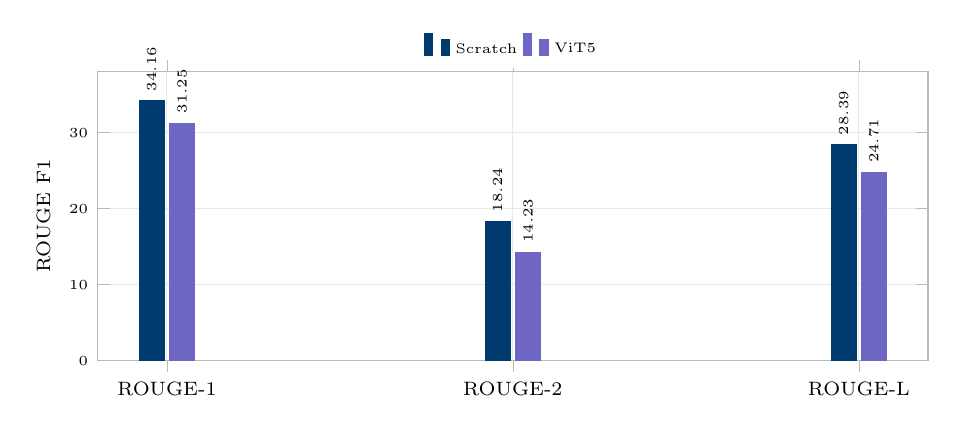
\begin{tikzpicture}
        \begin{axis}[
          width=\linewidth,height=5.25cm,
          ybar,bar width=9pt,
          ymin=0,ymax=38,
          symbolic x coords={R1,R2,RL},xtick=data,
          xticklabels={ROUGE-1,ROUGE-2,ROUGE-L},
          x tick label style={font=\scriptsize},yticklabel style={font=\tiny},
          ylabel={ROUGE F1},ylabel style={font=\scriptsize},
          legend style={font=\tiny,at={(0.5,1.01)},anchor=south,legend columns=2,draw=none},
          nodes near coords,nodes near coords style={font=\tiny,rotate=90,anchor=west},
          grid=major,grid style={gray!18},axis line style={gray!55},tick style={gray!55}]
          \addplot[fill=DeepBlue,draw=DeepBlue] coordinates {(R1,34.1597) (R2,18.2425) (RL,28.3899)};
          \addplot[fill=VitPurple,draw=VitPurple] coordinates {(R1,31.2495) (R2,14.2283) (RL,24.7108)};
          \legend{Scratch,ViT5}
        \end{axis}
      \end{tikzpicture}
    \column{0.43\textwidth}
      \textbf{Khoảng cách Scratch $-$ ViT5:}
      \vspace{1mm}
      \begin{tabular}{lr}
        \toprule
        \textbf{Thước đo} & \textbf{$\Delta$ điểm}\\
        \midrule
        ROUGE-1 & \textbf{+2,9102}\\
        ROUGE-2 & \textbf{+4,0142}\\
        ROUGE-L & \textbf{+3,6791}\\
        \bottomrule
      \end{tabular}
      \vspace{2mm}
      \begin{itemize}\small\tightitems
        \item R-2 tăng mạnh nhất: Scratch khớp tốt hơn ở mức cụm hai token.
        \item Scratch cũng sinh dài hơn: CR 9,7061\% so với 8,9242\%.
        \item Vì vậy cần xác nhận trên test và phân tích độ dài trước khi kết luận tổng quát.
      \end{itemize}
  \end{columns}
  \begin{keymessage}
    \scriptsize Validation ủng hộ Scratch Transformer, nhưng test độc lập mới quyết định liệu lợi thế này có bền vững hay không.
  \end{keymessage}
  \note{[Sources] Bảng validation do nhóm cung cấp. Các chênh lệch được tính trực tiếp từ bảng.}
\end{frame}

\begin{frame}{Compression ratio giúp đọc ROUGE đúng ngữ cảnh}
  \begin{columns}[T,onlytextwidth]
    \column{0.53\textwidth}
      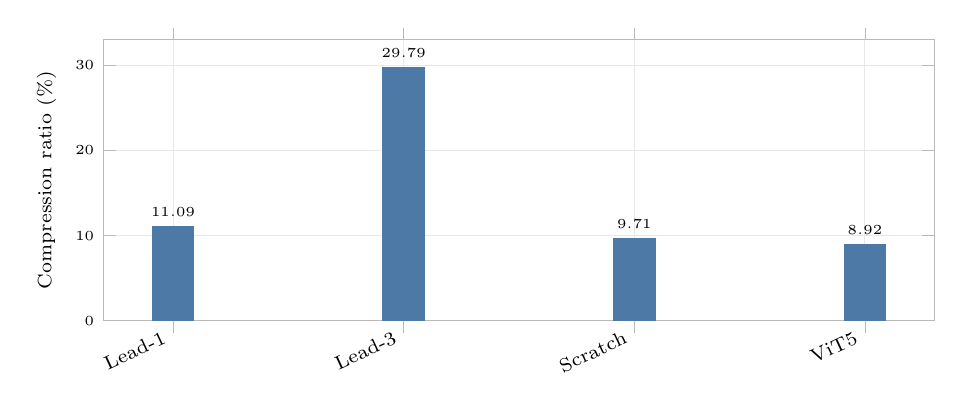
\begin{tikzpicture}
        \begin{axis}[
          width=\linewidth,height=5.15cm,
          ybar,bar width=15pt,
          ymin=0,ymax=33,
          symbolic x coords={Lead1,Lead3,Scratch,ViT5},xtick=data,
          xticklabels={Lead-1,Lead-3,Scratch,ViT5},
          x tick label style={rotate=25,anchor=east,font=\scriptsize},
          yticklabel style={font=\tiny},ylabel={Compression ratio (\%)},ylabel style={font=\scriptsize},
          nodes near coords,nodes near coords style={font=\tiny},
          grid=major,grid style={gray!18},axis line style={gray!55},tick style={gray!55}]
          \addplot[fill=MidBlue,draw=MidBlue] coordinates {(Lead1,11.0935) (Lead3,29.7882) (Scratch,9.7061) (ViT5,8.9242)};
        \end{axis}
      \end{tikzpicture}
    \column{0.44\textwidth}
      \textbf{Cách diễn giải:}
      \begin{itemize}\small\setlength{\itemsep}{4pt}
        \item \textbf{Lead-3} dài nhất nhưng ROUGE thấp nhất: thêm nhiều câu đầu không bảo đảm đúng trọng tâm.
        \item \textbf{ViT5} súc tích nhất trong hai mô hình sinh.
        \item \textbf{Scratch} dài hơn ViT5 khoảng 0,78 điểm phần trăm và đạt ROUGE cao hơn.
        \item ROUGE cần được đọc cùng độ dài, repetition và ví dụ đầu ra.
      \end{itemize}
      \vspace{1mm}
      \begin{softbox}
        \scriptsize CR ở đây được tính theo tỉ lệ độ dài tóm tắt sinh ra so với bài báo nguồn trên cùng tập validation.
      \end{softbox}
  \end{columns}
  \note{[Sources] Bảng validation do nhóm cung cấp.}
\end{frame}

\begin{frame}{Hai cấu hình được đóng băng trước khi chạy test}
  \begin{columns}[T,onlytextwidth]
    \column{0.49\textwidth}
      \begin{tcolorbox}[
        title=Scratch Transformer,
        colback=SoftBlue,colframe=DeepBlue,
        colbacktitle=DeepBlue,coltitle=white,fonttitle=\bfseries]
        \small
        \textbf{Cấu hình:} Beam-4, LP=1,1, nr=3\par
        \vspace{1mm}
        \begin{itemize}\tightitems
          \item Checkpoint tốt nhất: epoch 17
          \item Tokenizer: SentencePiece Unigram 16K
          \item Beam size: 4
          \item Length penalty: 1,1
          \item No-repeat n-gram: 3
        \end{itemize}
      \end{tcolorbox}
    \column{0.49\textwidth}
      \begin{tcolorbox}[
        title=ViT5-Base,
        colback=white,colframe=VitPurple,
        colbacktitle=VitPurple,coltitle=white,fonttitle=\bfseries]
        \small
        \textbf{Cấu hình:} beam4\_lp1.1\_max128\_nr3\par
        \vspace{1mm}
        \begin{itemize}\tightitems
          \item Model: \texttt{VietAI/vit5-base-}
                \texttt{vietnews-summarization}
          \item Beam size: 4
          \item Length penalty: 1,1
          \item Max new tokens: 128
          \item No-repeat n-gram: 3
        \end{itemize}
      \end{tcolorbox}
  \end{columns}
  \vspace{0.15cm}
  \begin{keymessage}[Điểm khóa của thực nghiệm]
    Sau slide này, mọi kết quả test phải được sinh bằng đúng hai cấu hình trên. Không điều chỉnh cấu hình sau khi xem test.
  \end{keymessage}
  \note{[Sources] Bảng validation do nhóm cung cấp; PROJECT\_BRIEF.md.}
\end{frame}

% ================================================================
% THAY THẾ TOÀN BỘ SLIDE 19--26 TRONG main.tex BẰNG KHỐI NÀY
% Yêu cầu: biên dịch bằng XeLaTeX; dùng đúng các package/màu/macro
% đã có trong main.tex hiện tại.
% ================================================================

% ----------------------------------------------------------------
% SLIDE 19
% ----------------------------------------------------------------
\begin{frame}{Đánh giá hai tầng: ROUGE và LLM judge}
  \begin{columns}[T,onlytextwidth]
    \column{0.48\textwidth}
      \begin{tcolorbox}[
        title=Đánh giá tự động trên toàn bộ test,
        colback=SoftGreen,colframe=GoodGreen,
        colbacktitle=GoodGreen,coltitle=white,
        fonttitle=\bfseries]
        \footnotesize
        \textbf{2.000 source $\times$ 4 hệ thống}
        \begin{itemize}\setlength{\itemsep}{1pt}
          \item ROUGE-1/2/L F1 theo cùng pipeline Unicode
          \item Compression ratio và độ dài đầu ra
          \item Cùng ID, cùng evaluator, cấu hình đã đóng băng
        \end{itemize}
        \textbf{Hỏi:} Prediction giống reference đến mức nào?
      \end{tcolorbox}

    \column{0.48\textwidth}
      \begin{tcolorbox}[
        title=Đánh giá source-grounded bằng LLM,
        colback=SoftBlue,colframe=MidBlue,
        colbacktitle=MidBlue,coltitle=white,
        fonttitle=\bfseries]
        \footnotesize
        \textbf{200 source $\times$ 4 hệ thống}
        \begin{itemize}\setlength{\itemsep}{1pt}
          \item 20 batch, mỗi batch gồm 10 source
          \item Ẩn tên hệ thống và không cung cấp reference
          \item Chấm 5 tiêu chí và gắn nhãn lỗi factuality
        \end{itemize}
        \textbf{Hỏi:} Tóm tắt có đúng, đủ và dễ đọc so với source không?
      \end{tcolorbox}
  \end{columns}

  \vspace{1mm}
  \begin{keymessage}[Nguyên tắc diễn giải]
    \scriptsize ROUGE và LLM judge là hai nguồn bằng chứng bổ sung; không thước đo nào tự nó đủ để kết luận chất lượng tóm tắt.
  \end{keymessage}
  \note{[Sources] Giao thức test\_core\_2000; giao thức LLM-as-a-Judge của nhóm; 20 batch đánh giá, 200 source và 800 candidate summaries.}
\end{frame}

% ----------------------------------------------------------------
% SLIDE 20
% ----------------------------------------------------------------
\begin{frame}{ROUGE ưu tiên Scratch Transformer trên 2.000 mẫu}
  \begin{columns}[T,onlytextwidth]
    \column{0.54\textwidth}
      \textbf{Kết quả trên toàn bộ tập test:}
      \vspace{1mm}

      \resizebox{\linewidth}{!}{%
        \begin{tabular}{lrrrrr}
          \toprule
          \textbf{Hệ thống} & \textbf{N} & \textbf{R-1} & \textbf{R-2} & \textbf{R-L} & \textbf{CR (\%)}\\
          \midrule
          Lead-1              & 2.000 & 26,78 & 12,17 & 20,80 & 11,51\\
          Lead-3              & 2.000 & 25,12 & 11,03 & 17,92 & 30,14\\
          \rowcolor{SoftYellow}
          \textbf{Scratch Transformer} & \textbf{2.000} & \textbf{33,84} & \textbf{17,84} & \textbf{28,30} & 9,42\\
          ViT5-Base           & 2.000 & 31,22 & 14,51 & 25,00 & 8,63\\
          \bottomrule
        \end{tabular}
      }

      \vspace{2.5mm}
      \begin{softbox}
        \small
        \textbf{Quan sát:} Scratch đạt ROUGE cao nhất trên cả ba thước đo; ViT5 đứng thứ hai. Lead-3 sinh dài nhất nhưng có ROUGE thấp hơn Lead-1.
      \end{softbox}

      \vspace{1.5mm}
      \begin{keymessage}[Kết luận theo ROUGE]
        \scriptsize Scratch có độ trùng với reference cao nhất. Kết quả này chưa chứng minh prediction đúng sự thật, bao phủ đủ ý hay không chứa thông tin suy diễn.
      \end{keymessage}

    \column{0.43\textwidth}
      \vspace{0.70cm}
      \centering
      \maybeimage[\linewidth]
        {figures/test_rouge_chart.pdf}
        {4.35cm}
        {Biểu đồ ROUGE trên test}

      \vspace{1mm}
      {\scriptsize\color{MutedGray}
        Thước đo chính: mức trùng n-gram với reference.}
  \end{columns}
  \note{[Sources] Kết quả đánh giá tự động trên test\_core\_2000; 2.000 prediction hợp lệ cho mỗi hệ thống.}
\end{frame}

% ----------------------------------------------------------------
% SLIDE 21
% ----------------------------------------------------------------
\begin{frame}{LLM judge mù danh tính đánh giá trực tiếp theo source}
  \begin{columns}[T,onlytextwidth]
    \column{0.54\textwidth}
      \begin{softbox}
        \footnotesize
        \textbf{1. Input}\par
        01 source $+$ 04 candidate summaries ký hiệu A/B/C/D.
        \vspace{1.2mm}\par
        \textbf{2. Làm mù và cân bằng}\par
        Ẩn tên mô hình, bỏ reference; mỗi hệ thống xuất hiện 50 lần tại từng vị trí A/B/C/D.
        \vspace{1.2mm}\par
        \textbf{3. Output có cấu trúc}\par
        Điểm 1--5, Overall có trọng số, cờ major factual error và loại lỗi.
      \end{softbox}

      \vspace{1.5mm}
      \begin{greenbox}
        \centering\footnotesize
        \textbf{20 batch $\times$ 10 source = 200 source}\par
        4 hệ thống $\times$ 200 source = \textbf{800 summaries}
      \end{greenbox}

    \column{0.42\textwidth}
      \textbf{Rubric chấm điểm:}
      \vspace{1mm}
      \renewcommand{\arraystretch}{1.32}
      \begin{tabularx}{\linewidth}{Xr}
        \toprule
        \textbf{Tiêu chí} & \textbf{Trọng số}\\
        \midrule
        Faithfulness                  & 35\%\\
        Coverage                      & 25\%\\
        Focus                         & 15\%\\
        Fluency                       & 15\%\\
        Conciseness                   & 10\%\\
        \bottomrule
      \end{tabularx}
  \end{columns}

  \vspace{1mm}
  \begin{keymessage}[Vai trò của LLM judge]
    \scriptsize Đây là phép đánh giá bổ sung dựa trên source, không phải ground truth và không thay thế hoàn toàn đánh giá của con người.
  \end{keymessage}
  \note{[Sources] Prompt LLM-as-a-Judge; secret mapping; thống kê cân bằng vị trí A/B/C/D từ pipeline phân tích.}
\end{frame}

% ----------------------------------------------------------------
% SLIDE 22
% ----------------------------------------------------------------
\begin{frame}{LLM judge đảo thứ hạng: Lead-3 dẫn đầu}
  \begin{columns}[T,onlytextwidth]
    \column{0.58\textwidth}
      \textbf{Điểm Overall trung bình và bootstrap 95\% CI:}
      \vspace{-1mm}
      \begin{center}
      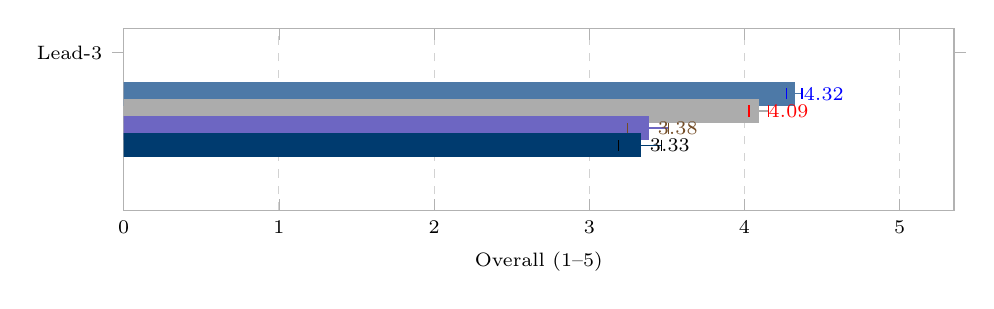
\begin{tikzpicture}
        \begin{axis}[
          xbar,
          xmin=0,xmax=5.35,
          width=\linewidth,height=3.90cm,
          bar width=8pt,
          symbolic y coords={Scratch,ViT5,Lead-1,Lead-3},
          ytick=data,
          yticklabel style={font=\scriptsize},
          xtick={0,1,2,3,4,5},
          xticklabel style={font=\scriptsize},
          xlabel={Overall (1--5)},
          xlabel style={font=\scriptsize},
          xmajorgrids=true,
          grid style={dashed,gray!35},
          axis line style={gray!60},
          tick style={gray!60},
          nodes near coords,
          nodes near coords align={horizontal},
          every node near coord/.append style={font=\scriptsize},
          enlarge y limits=0.18,
        ]
          \addplot+[fill=MidBlue,draw=MidBlue,error bars/.cd,x dir=both,x explicit]
            coordinates {(4.320,Lead-3) +- (0.051,0)};
          \addplot+[fill=gray!65,draw=gray!65,error bars/.cd,x dir=both,x explicit]
            coordinates {(4.093,Lead-1) +- (0.064,0)};
          \addplot+[fill=VitPurple,draw=VitPurple,error bars/.cd,x dir=both,x explicit]
            coordinates {(3.379,ViT5) +- (0.130,0)};
          \addplot+[fill=DeepBlue,draw=DeepBlue,error bars/.cd,x dir=both,x explicit]
            coordinates {(3.328,Scratch) +- (0.139,0)};
        \end{axis}
      \end{tikzpicture}
      \end{center}

    \column{0.38\textwidth}
      \textbf{Major factual error:}
      \vspace{1mm}
      \scriptsize
      \renewcommand{\arraystretch}{1.22}
      \begin{tabularx}{\linewidth}{Xr}
        \toprule
        \textbf{Hệ thống} & \textbf{Tỷ lệ}\\
        \midrule
        Lead-3  & 0/200 quan sát\\
        Lead-1  & 0/200 quan sát\\
        Scratch & 91/200 = 45,5\%\\
        ViT5    & 104/200 = 52,0\%\\
        \bottomrule
      \end{tabularx}

      \vspace{1.2mm}
      \begin{softbox}
        \RaggedRight\scriptsize
        \textbf{Lead-3 vs Lead-1:} $+0{,}226$, CI $[0{,}168;\,0{,}289]$.\par
        \vspace{0.8mm}
        \textbf{ViT5 vs Scratch:} $+0{,}052$, CI $[-0{,}125;\,0{,}229]$; chưa khác biệt rõ.
      \end{softbox}
  \end{columns}

  \vspace{0.7mm}
  \begin{keymessage}[Kết luận theo rubric hiện tại]
    \scriptsize Lead-3 đạt Overall cao nhất trên 200 mẫu; ViT5 và Scratch tương đương trong phạm vi mẫu thay vì có một mô hình thắng rõ ràng.
  \end{keymessage}
  \note{[Sources] Kết quả phân tích LLM judge: điểm hệ thống, bootstrap confidence intervals, paired comparison và major factual error rates. Với hai baseline, 0/200 là tỷ lệ quan sát, không phải khẳng định xác suất lỗi trong tổng thể bằng 0.}
\end{frame}

% ----------------------------------------------------------------
% SLIDE 23
% ----------------------------------------------------------------
\begin{frame}{Mô hình sinh súc tích, nhưng factuality là điểm nghẽn}
  \begin{columns}[T,onlytextwidth]
    \column{0.60\textwidth}
      \textbf{Điểm trung bình theo từng tiêu chí:}
      \vspace{1mm}
      \resizebox{\linewidth}{!}{%
        \renewcommand{\arraystretch}{1.38}
        \begin{tabular}{lrrrrr}
          \toprule
          \textbf{Hệ thống} & \textbf{Faith.} & \textbf{Cover.} & \textbf{Focus} & \textbf{Fluency} & \textbf{Concise}\\
          \midrule
          Lead-1  & \cellcolor{SoftGreen}4,995 & 2,420 & 4,060 & \cellcolor{SoftGreen}4,710 & 4,245\\
          Lead-3  & \cellcolor{SoftGreen}\textbf{5,000} & \cellcolor{SoftGreen}\textbf{3,415} & \cellcolor{SoftGreen}\textbf{4,145} & 4,630 & 3,995\\
          Scratch & 3,385 & 2,155 & 3,620 & 4,095 & 4,470\\
          ViT5    & 3,255 & 2,220 & 3,810 & 4,340 & \cellcolor{SoftGreen}\textbf{4,625}\\
          \bottomrule
        \end{tabular}
      }

      \vspace{1.5mm}
      {\footnotesize
      \begin{itemize}\setlength{\itemsep}{1pt}
        \item Lead-3 dẫn đầu nhờ Faithfulness và Coverage.
        \item ViT5 trôi chảy và súc tích hơn Scratch.
        \item Hai mô hình sinh vẫn thấp hơn rõ ở Faithfulness.
      \end{itemize}}

    \column{0.37\textwidth}
      \textbf{Ba loại lỗi phổ biến nhất:}
      \vspace{1mm}
      \begin{tcolorbox}[
        title=Scratch Transformer,
        colback=SoftBlue,colframe=DeepBlue,
        colbacktitle=DeepBlue,coltitle=white,
        fonttitle=\bfseries,
        left=1mm,right=1mm,top=0.7mm,bottom=0.7mm]
        \scriptsize
        \begin{enumerate}\tightitems
          \item Sai quan hệ: \textbf{30,5\%}
          \item Sai predicate: \textbf{24,5\%}
          \item Không được source hỗ trợ: \textbf{18,0\%}
        \end{enumerate}
      \end{tcolorbox}
      \vspace{1mm}
      \begin{tcolorbox}[
        title=ViT5-Base,
        colback=white,colframe=VitPurple,
        colbacktitle=VitPurple,coltitle=white,
        fonttitle=\bfseries,
        left=1mm,right=1mm,top=0.7mm,bottom=0.7mm]
        \scriptsize
        \begin{enumerate}\tightitems
          \item Không được source hỗ trợ: \textbf{31,0\%}
          \item Sai predicate: \textbf{25,0\%}
          \item Sai ngày/thời gian: \textbf{21,5\%}
        \end{enumerate}
      \end{tcolorbox}
  \end{columns}

  \vspace{0.6mm}
  \begin{keymessage}[Trade-off chính]
    \scriptsize Fluency và Conciseness tốt không bù được rủi ro factuality; cải thiện tiếp theo cần tập trung vào độ trung thực với source.
  \end{keymessage}
  \note{[Sources] llm\_judge\_analysis\_outputs: criterion means và factual error type rates cho từng hệ thống.}
\end{frame}

% ----------------------------------------------------------------
% SLIDE 24
% ----------------------------------------------------------------
\begin{frame}{ROUGE và LLM judge trả lời hai câu hỏi khác nhau}
  \begin{columns}[T,onlytextwidth]
    \column{0.48\textwidth}
      \begin{tcolorbox}[
        title=ROUGE trên 2.000 mẫu,
        colback=SoftGreen,colframe=GoodGreen,
        colbacktitle=GoodGreen,coltitle=white,
        fonttitle=\bfseries]
        \footnotesize
        \textbf{Đo:} mức trùng n-gram với reference.

        \vspace{0.7mm}
        \textbf{Xếp hạng:}\par
        \textbf{Scratch $>$ ViT5 $>$ Lead-1 $>$ Lead-3}

        \vspace{0.7mm}
        \textbf{Cho thấy:}\par
        Scratch tái tạo từ ngữ và nội dung của reference tốt nhất.

        \vspace{0.7mm}
        \textbf{Giới hạn:}\par
        Nhạy với cách diễn đạt, reference nhiễu và lead bias.
      \end{tcolorbox}

    \column{0.48\textwidth}
      \begin{tcolorbox}[
        title=LLM judge trên 200 mẫu,
        colback=SoftBlue,colframe=MidBlue,
        colbacktitle=MidBlue,coltitle=white,
        fonttitle=\bfseries]
        \footnotesize
        \textbf{Đo:} mức đúng, đủ và tập trung so với source.

        \vspace{0.7mm}
        \textbf{Xếp hạng:}\par
        \textbf{Lead-3 $>$ Lead-1 $>$ ViT5 $\approx$ Scratch}

        \vspace{0.7mm}
        \textbf{Cho thấy:}\par
        Baseline trích xuất giữ thông tin đáng tin cậy hơn trong rubric hiện tại.

        \vspace{0.7mm}
        \textbf{Giới hạn:}\par
        Có thể chịu thiên lệch độ dài, extractive bias và đặc tính của judge.
      \end{tcolorbox}
  \end{columns}

  \vspace{0.8mm}
  \begin{keymessage}[Tổng hợp bằng chứng]
    \scriptsize Scratch khớp reference tốt nhất nhưng không đáng tin cậy nhất theo LLM judge. Sự đảo thứ hạng cho thấy kết luận phụ thuộc trực tiếp vào câu hỏi mà thước đo đang trả lời.
  \end{keymessage}
  \note{[Sources] Kết quả ROUGE trên test\_core\_2000 và kết quả LLM-as-a-Judge trên 200 source. Hai phép đo dùng cỡ mẫu khác nhau nên được báo cáo song song, không gộp thành một mẫu chung.}
\end{frame}

% ----------------------------------------------------------------
% SLIDE 25
% ----------------------------------------------------------------
\begin{frame}{LLM judge bổ sung bằng chứng, nhưng chưa phải ground truth}
  \scriptsize
  \renewcommand{\arraystretch}{1.27}
  \setlength{\tabcolsep}{4.0pt}
  \begin{tabularx}{\textwidth}{>{\bfseries\RaggedRight\arraybackslash}p{2.75cm}X X}
    \toprule
    \textbf{Đã kiểm soát} & \textbf{Rủi ro còn lại} & \textbf{Cách kiểm chứng}\\
    \midrule
    Ẩn tên hệ thống và reference
      & Judge vẫn có thể ưu tiên văn bản trích xuất hoặc cách viết quen thuộc
      & Human audit 30--50 mẫu, ưu tiên các mẫu bị gắn major factual error\\
    \rowcolor{LightGray}
    Cân bằng vị trí A/B/C/D
      & Một judge và thao tác qua giao diện chat chưa bảo đảm tính lặp lại tuyệt đối
      & Chấm lại một tập con bằng judge thứ hai hoặc hoán đổi thứ tự candidate\\
    Cùng rubric và cùng 200 source
      & Coverage có thể tăng đơn giản vì output dài hơn
      & Tính CR trên đúng 200 mẫu; phân tích tương quan CR--Coverage và CR--Conciseness\\
    \rowcolor{LightGray}
    Bootstrap và paired comparison
      & 200 mẫu nhỏ hơn toàn bộ test 2.000 mẫu
      & Báo cáo rõ cỡ mẫu; mở rộng đánh giá nếu tài nguyên cho phép\\
    \bottomrule
  \end{tabularx}

  \vspace{1.2mm}
  \begin{softbox}
    \small
    \textbf{Biến nhiễu cần kiểm tra:} trên 2.000 mẫu, CR của Lead-1/Lead-3/Scratch/ViT5 lần lượt là \textbf{11,5\% / 30,1\% / 9,4\% / 8,6\%}. Không nên dùng trực tiếp các giá trị này để giải thích điểm LLM trước khi tính lại trên đúng tập con 200 mẫu.
  \end{softbox}

  \vspace{0.7mm}
  \begin{keymessage}[Cách diễn đạt an toàn]
    \scriptsize Lead-3 tốt nhất theo rubric LLM hiện tại trên 200 mẫu; kết luận cần được xem là bằng chứng bổ sung và nên được kiểm chứng bằng đánh giá người.
  \end{keymessage}
  \note{[Sources] Giao thức LLM-as-a-Judge; thống kê position balance; compression ratio trên test\_core\_2000; phân tích giới hạn của thiết kế đánh giá.}
\end{frame}

% ----------------------------------------------------------------
% SLIDE 26
% ----------------------------------------------------------------
\begin{frame}{Kết luận: không có hệ thống thắng trên mọi tiêu chí}
  \vspace{0.12cm}
  \begin{columns}[T,onlytextwidth]
    \column{0.31\textwidth}
      \centering
      {\color{DeepBlue}\Huge\bfseries 01}\par\vspace{1mm}
      {\bfseries ROUGE}\par
      \small Scratch đạt độ trùng với reference cao nhất trên 2.000 mẫu test.

    \column{0.31\textwidth}
      \centering
      {\color{DeepBlue}\Huge\bfseries 02}\par\vspace{1mm}
      {\bfseries LLM judge}\par
      \small Lead-3 dẫn đầu trên 200 mẫu; ViT5 và Scratch chưa khác rõ về Overall.

    \column{0.31\textwidth}
      \centering
      {\color{DeepBlue}\Huge\bfseries 03}\par\vspace{1mm}
      {\bfseries Bài học đánh giá}\par
      \small Độ trùng, độ dài, factuality và đánh giá người phải được đọc cùng nhau.
  \end{columns}

  \vspace{0.36cm}
  \begin{keymessage}[Kết luận trung tâm]
    \centering\small
    Scratch khớp reference tốt nhất; Lead-3 mạnh nhất theo LLM source-grounded hiện tại; ViT5 diễn đạt trôi chảy và súc tích hơn Scratch nhưng chưa vượt rõ về Overall. Vì vậy, một điểm ROUGE đơn lẻ không đủ để kết luận chất lượng tóm tắt.
  \end{keymessage}

  \vfill
  \centering
  {\color{DeepBlue}\Large\bfseries Cảm ơn thầy cô và các bạn đã lắng nghe!}\par
  \vspace{1mm}
  {\bfseries \MemberNames}
  \note{[Sources] Tổng hợp kết quả ROUGE, LLM-as-a-Judge, bootstrap paired comparison và phân tích lỗi của dự án.}
\end{frame}
\end{document}
